%!TEX root=../../main.tex
\begin{chapterpage}{Two-sample Hypothesis testing}
  \chaptertitle{Two-sample Hypothesis testing}
  \label{inferenceForTwoSample}
  % \chaptersection{oneSampleMeansWithTDistribution}
  \chaptersection{differenceOfTwoProportions}
  \chaptersection{pairedData}
  \chaptersection{TwoVariancesSection}
  \chaptersection{differenceOfTwoMeansEqualVar}
  \chaptersection{differenceOfTwoMeans}
  %\chaptersection{PowerForDifferenceOfTwoMeans}
  %\chaptersection{anovaAndRegrWithCategoricalVariables}
  \chaptersection{inferenceForNumericalDataNotes}
  %\chaptersection{inferenceForNumericalDataExercises}
\end{chapterpage}
\renewcommand{\chapterfolder}{ch_inference_for_means_oi_biostat}

\chapterintro{
%  Chapter~\ref{foundationsForInference} introduced some primary tools of statistical inference\textemdash point estimates, interval estimates, and hypothesis tests. This chapter discusses settings where these tools are often used, including the analysis of paired observations and the comparison of two or more independent groups. The chapter also covers the important topic of estimating an appropriate sample size when a study is being designed.  The chapter starts with introducing a new distribution, the $t$-distribution, which can be used for small sample sizes.

Chapter~\ref{confidenceIntervals} and~\ref{ch:OneSampleHT} introduced a framework for statistical inference based on confidence intervals and hypotheses. In this chapter, we encounter several new point estimates and scenarios. In contrast with the previous situation, there is not a reference value, but a comparison between two groups. In each case, the inference ideas remain the same:
\begin{enumerate}
\setlength{\itemsep}{0mm}
\item Determine which point estimate or test statistic is useful.
\item Identify an appropriate distribution for the point estimate or test statistic.
\end{enumerate}

}


%__________________

\section{Inference for the difference of two proportions}
\label{differenceOfTwoProportions}


Just as inference can be done for the difference of two population means, conclusions can also be drawn about the difference of two population proportions: $p_1 - p_2$. 

\subsection{Sampling distribution of the difference of two proportions}

\index{sampling distribution!difference of two proportions}
\index{point estimate!difference of two proportions}

The normal model can be applied to $\hat{p}_1 - \hat{p}_2$ if the sampling distribution for each sample proportion is nearly normal and if the samples are independent random samples from the relevant populations. 

\begin{onebox}{Conditions for the sampling distribution of $\hat{p}_1 - \hat{p}_2$ to be approximately normal}
The difference $\hat{p}_1 - \hat{p}_2$ tends to follow a normal model when
\begin{itemize}
\setlength{\itemsep}{0mm}
\item each of the two samples are random samples from a population,
\item the two samples are independent of each other, and
\item each sample proportion follows (approximately) a normal model. This condition is satisfied when $n_1p_1, n_1(1 - p_1), n_2 p_2$ and $n_2(1 - p_2)$ are all $\geq 10$.
\end{itemize}
The standard error of the difference in sample proportions is
\index{standard error (SE)!difference in proportions}
\begin{eqnarray}
SE_{\hat{p}_1 - \hat{p}_2}
	= \sqrt{SE_{\hat{p}_1}^2 + SE_{\hat{p}_2}^2}
	= \sqrt{\frac{p_1(1-p_1)}{n_1} + \frac{p_2(1-p_2)}{n_2}},
\label{seForDiffOfProp}
\end{eqnarray}
where $p_1$ and $p_2$ are the population proportions, and $n_1$ and $n_2$ are the two sample sizes.
\end{onebox}


%\textD{\newpage}


\subsection{Confidence intervals for $\pmb{\MakeLowercase{p_1 - p_2}}$}
\label{confidenceIntervalsDifferenceProportions}
\index{confidence interval!difference of two proportions}

When calculating confidence intervals for a difference of two proportions using the normal approximation to the binomial, the two sample proportions are used to verify the success-failure condition and to compute the standard error.

\begin{examplewrap}
\begin{nexample}{The way a question is phrased can influence a person's response. For example, Pew Research Center conducted a survey with the following question:\footnotemark{}
\begin{quote}
As you may know, by 2014 nearly all Americans will be required to have health insurance. [People who do not buy insurance will pay a penalty] while [People who cannot afford it will receive financial help from the government]. Do you approve or disapprove of this policy?
\end{quote}
\index{data!health care|(}For each randomly sampled respondent, the statements in brackets were randomized: either they were kept in the order given above, or the order of the two statements was reversed. Figure~\ref{pewPollResultsForRandomizedStatementOrdering} shows the results of this experiment. Calculate and interpret a 90\% confidence interval of the difference in the probability of approval of the policy.}
First the conditions for the use of a normal model must be verified. The Pew Research Center uses sampling methods that produce random samples of the US population (at least approximately) and because each group was a simple random sample from less than 10\% of the population, the observations are independent, both within the samples and between the samples. The success-failure condition also holds for each sample, so the normal model can be used for confidence intervals for the difference in approval proportions.  The point estimate of the difference in support, where $\hat{p}_1$ corresponds to the original ordering and $\hat{p}_2$ to the reversed ordering:
$$\hat{p}_{1} - \hat{p}_{2} = 0.47 - 0.34 = 0.13.$$
The standard error can be computed from Equation~\eqref{seForDiffOfProp} using the sample proportions:
$$SE \approx \sqrt{\frac{0.47(1-0.47)}{771} + \frac{0.34(1-0.34)}{732}} = 0.025.$$
For a 90\% confidence interval, $z^{\star} = 1.65$:
$$\text{point estimate} \ \pm\ z^{\star} \times SE \quad \to \quad 0.13 \ \pm\ 1.65 \times  0.025 \quad \to \quad (0.09, 0.17).$$
With 90\% confidence, the proportion approving the 2010 health care law ranged between 9\% and 17\% depending on the phrasing of the question. The Pew Research Center interpreted this modestly large difference as an indication that for most of the public, opinions were still fluid on the health insurance mandate.  The law eventually passed as the Affordable Health Care Act (ACA).
\index{data!health care|)}
\end{nexample}
\end{examplewrap}
\footnotetext{\oiRedirect{textbook-health_care_bill_2012}{www.people-press.org/2012/03/26/public-remains-split-on-health-care-bill-opposed-to-mandate}. Sample sizes for each polling group are approximate.}

\begin{figure}[h]
\centering
\begin{tabular}{c c c c c}
	& Sample size ($n_i$) & Approve (\%)	& Disapprove (\%)	& Other \\
\hline
Original ordering & 771	& 47	& 49	& 3 \\
Reversed ordering & 732	& 34	& 63	& 3 \\
\hline
\end{tabular}
\caption{Results for a Pew Research Center poll where the ordering of two statements in a question regarding healthcare were randomized.\vspaceB{-2mm}}
\label{pewPollResultsForRandomizedStatementOrdering}
\end{figure}


%\textD{\newpage}


\subsection{Hypothesis testing for $\pmb{\MakeLowercase{p_1 - p_2}}$}

%\index{hypothesis test!difference of two proportions}

Hypothesis tests for $p_1 - p_2$ are usually testing the null hypothesis of no difference between $p_1$ and $p_2$; i.e. $H_0:\,p_1 - p_2 = 0$. Under the null hypothesis, $\hat{p}_1 - \hat{p}_2$ is normally distributed with mean 0 and standard deviation $\sqrt{p(1-p)(\frac{1}{n_1} + \frac{1}{n_2})}$, where under the null hypothesis $p = p_1 = p_2$.

Since $p$ is unknown, an estimate is used to compute the standard error of $\hat{p}_1 - \hat{p}_2$; $p$ can be estimated by $\hat{p}$, the weighted average of the sample proportions $\hat{p}_1$ and $\hat{p}_2$:
\[\hat{p} = \dfrac{n_{1}\hat{p}_1 + n_{2}\hat{p}_2}{n_{1} + n_{2}} = \dfrac{x_{1} + x_{2}}{n_{1} + n_{2}}, \]
where $x_1$ is the number of observed events in the first sample and $x_2$ is the number of observed events in the second sample. This \term{pooled proportion} $\hat{p}$ is also used to check the success-failure condition.

The test statistic $z$ for testing $H_0:\, p_1 = p_2$ versus $H_A: p_1 \neq p_2$ equals:

\[z = \dfrac{\hat{p}_1 - \hat{p}_2}{\sqrt{\hat{p}(1-\hat{p})\left(\frac{1}{n_1} + \frac{1}{n_2} \right)}}. \]
 
\index{data!mammography|(}
\index{data!breast cancer|(}

\begin{examplewrap}
  \begin{nexample}{

\index{data!cancer in dogs, herbicide|(}
 We investigate whether there is an increased risk of cancer in dogs that are exposed to the herbicide 2,4-dichlorophenoxyacetic acid (2,4-D). A study in 1994 examined 491 dogs that had developed cancer and 945 dogs as a control group.\footnote{Hayes HM, Tarone RE, Cantor KP, Jessen CR, McCurnin DM, and Richardson RC. 1991. Case-Control Study of Canine Malignant Lymphoma: Positive Association With Dog Owner's Use of 2, 4-Dichlorophenoxyacetic Acid Herbicides. Journal of the National Cancer Institute 83(17):1226-1231.} Of these two groups, researchers identified which dogs had been exposed to 2,4-D in their owner's yard. The results are shown in Table~\ref{24DAndCancerInDogs}.


}

Is this study an experiment or an observational study? The owners were not instructed to apply or not apply the herbicide, so this is an observational study. This question was especially tricky because one group was called the \emph{control group}, which is a term usually seen in experiments.

Set up hypotheses to test whether 2,4-D and the occurrence of cancer in dogs are related. Use a one-sided test and compare across the cancer and no cancer groups. Using the proportions within the cancer and no cancer groups may seem odd. We intuitively may desire to compare the fraction of dogs with cancer in the 2,4-D and no 2,4-D groups, since the herbicide is an explanatory variable. However, the cancer rates in each group do not necessarily reflect the cancer rates in reality due to the way the data were collected. For this reason, computing cancer rates may greatly alarm dog owners. \\
$H_0$: the proportion of dogs with exposure to 2,4-D is the same in ``cancer'' and ``no cancer'' dogs, $p_c - p_n = 0$. \\
$H_A$: dogs with cancer are more likely to have been exposed to 2,4-D than dogs without cancer, $p_c - p_n > 0$.


Under the assumption of independence, we can use the normal model and make statements regarding the canine population based on the data.

The point estimate of the difference in sample proportions is $\hat{p}_c - \hat{p}_n = 0.067$. First, we   compute the pooled proportion:
$$\hat{p} = \frac{\text{\# of ``successes''}}{\text{\# of cases}} = \frac{191 + 304}{191+300+304+641} = 0.345$$

%\begin{termBox}{\tBoxTitle{Pooled estimate of a proportion}

The estimate for the standard error is $SE = 0.026$. 
Compute the test statistic:
\begin{eqnarray*}
z = \frac{\text{point estimate} - \text{null value}}{SE} = \frac{0.067 - 0}{0.026} = 2.58
\end{eqnarray*}
We leave the picture to you. Looking up $z=2.58$ in the normal probability table: 0.9951. However this is the lower tail, and the upper tail represents the p-value: $1-0.9951 = 0.0049$. We reject the null hypothesis and conclude that dogs getting cancer and owners using 2,4-D are associated.
    \end{nexample}
\end{examplewrap}
\begin{table}[h]
\centering
\begin{tabular}{rrr}
  \hline
 & cancer & no cancer \\
  \hline
2,4-D & 191 & 304 \\
no 2,4-D & 300 & 641 \\
   \hline
\end{tabular}
\caption{Summary results for cancer in dogs and the use of 2,4-D by the dog's owner.}
\label{24DAndCancerInDogs}
\end{table}
\begin{examplewrap}
\begin{nexample}{The use of screening mammograms for breast cancer has been controversial for decades because the overall benefit on breast cancer mortality is uncertain.  Several large randomized studies have been conducted in an attempt to estimate the effect of mammogram screening. A 30-year study to investigate the effectiveness of mammograms versus a standard non-mammogram breast cancer exam was conducted in Canada with 89,835 female participants.\footnotemark{} During a 5-year screening period, each woman was randomized to either receive annual mammograms or standard physical exams for breast cancer.  During the 25 years following the screening period, each woman was screened for breast cancer according to the standard of care at her health care center. \vspace{3mm}

At the end of the 25 year follow-up period, 1,005 women died from breast cancer. The results by intervention are summarized in Figure~\ref{mammogramStudySummaryTable}. \vspace{3mm}

Assess whether the normal model can be used to analyze the study results.}\label{mammogramSuccessFailure}%

Since the participants were randomly assigned to each group, the groups can be treated as independent, and it is reasonable to assume independence of patients within each group.  Participants in randomized studies are rarely random samples from a population, but the investigators in the Canadian trial recruited  participants using a general publicity campaign, by sending personal invitation letters to women identified from general population lists, and through contacting family doctors.  In this study, the participants can reasonably be thought of as a random sample.

The pooled proportion $\hat{p}$ is  

\[\hat{p} = \dfrac{x_{1} + x_{2}}{n_{1} + n_{2}} = \dfrac{500 + 505}{500 + 44,425 + 505 + 44,405} = 0.0112. \]

Checking the success-failure condition for each group: 
\begin{align*}
\hat{p} \times n_{mgm} &= 0.0112 \times \text{44,925} = 503
& (1 - \hat{p}) \times n_{mgm} &= 0.9888 \times \text{44,925} = \text{44,422} \\
\hat{p} \times n_{ctrl} &= 0.0112 \times \text{44,910} = 503
& (1 - \hat{p}) \times n_{ctrl} &= 0.9888 \times \text{44,910} = \text{44,407}
\end{align*}
All values are at least 10. 

The normal model can be used to analyze the study results.
\end{nexample}
\end{examplewrap}
\footnotetext{\oiRedirect{textbook-90k_mammogram_study_2014}{Miller AB. 2014. \emph{Twenty five year follow-up for breast cancer incidence and mortality of the Canadian National Breast Screening Study: randomised screening trial}. BMJ 2014;348:g366 doi: 10.1136/bmj.g366}}

\begin{figure}[h]
	\centering
	\begin{tabular}{rrcc}
		& \multicolumn{3}{c}{Death from breast cancer?} \\
		\cline{2-4}
		& \ \hspace{3mm}\ & Yes & No \\
		\hline
		Mammogram && 500 & 44,425 \\
		Control && 505 & 44,405 \\
		\hline
	\end{tabular}
	\caption{Summary results for the mammogram study.}
	\label{mammogramStudySummaryTable}
\end{figure}

%\textD{\newpage}

\begin{examplewrap}
\begin{nexample}{Do the results from the study provide convincing evidence of a difference in the proportion of breast cancer deaths between women who had annual mammograms during the screening period versus women who received annual screening with physical exams?}\label{mammogramExProp}%
The null hypothesis is that the probability of a breast cancer death is the same for the women in the two groups. If group 1 represents the mammogram group and group 2 the control group, $H_0: p_1 = p_2$ and $H_A: p_1 \neq p_2$.  Let $\alpha = 0.05$.

Calculate the test statistic $z$:
\[z = \dfrac{0.01113 - 0.01125}{\sqrt{(0.0112)(1-0.0112)\left(\frac{1}{44,925} + \frac{1}{44,910} \right)}} = -0.17.
\]	
The two-sided $p$-value is $P|Z| \ge 0.17 = 0.8650$,  which is greater than 0.05. There is insufficient evidence to reject the null hypothesis; the observed difference in breast cancer death rates is reasonably explained by chance. 	

Evaluating medical treatments typically requires accounting for additional evidence that cannot be evaluated from a statistical test. For example, if mammograms are much more expensive than a standard screening and do not offer clear benefits, there is reason to recommend standard screenings over mammograms. This study also found that a higher proportion of diagnosed breast cancer cases in the mammogram screening arm (3250 in the mammogram group vs 3133 in the physical exam group), despite the nearly equal number of breast cancer deaths.  The investigators inferred that mammograms may cause over-diagnosis of breast cancer, a phenomenon in which a breast cancer diagnosed with mammogram and subsequent biopsy may never become symptomatic. The possibility of over-diagnosis is one of the reasons mammogram screening remains controversial.
\end{nexample}
\end{examplewrap}

\begin{examplewrap}
\begin{nexample}{Calculate a 95\% confidence interval for the difference in proportions of deaths from breast cancer from the Canadian study.}\label{mammogramExConfInt}%

The independence and random sampling conditions have already been discussed.  The success failure condition should be checked for each sample, since this is not a hypothesis testing context (i.e., there is no null hypothesis). For the mammogram group, $\hat{p}_1 = 0.01113$; $n_1 \hat{p}_1 = (0.1113)(44,925) = 500$ and $n_1 (1 - \hat{p}_1) = 39,925.$ It is easy to show that the success failure condition is holds for the control group as well.

The point estimate for the difference in the probability of death is
$$\hat{p}_{1} - \hat{p}_{2} = 0.01113 - 0.01125 = -0.00012,$$ or 0.012\%.

The standard error for the estimated difference uses the individual estimates of the probability of a death:
$$SE \approx \sqrt{\frac{0.01113(1-0.01113)}{44,925} + \frac{0.01125(1-0.01125)}{44,910}} = 0.0007. $$

The 95\% confidence interval is given by 
$$ -0.00012 \pm (1.96) (0.0007) = (-0.0015, 0.0013).$$

With 95\% confidence, the difference in the probability of death is between -0.15\% and 0.13\%. As expected from the large $p$-value, the confidence interval contains the null value 0.
\end{nexample}
\end{examplewrap}

\index{data!breast cancer|)}
\index{data!mammography|)}




%___________
\section{Two-sample test for paired data}
\label{pairedData}

\index{paired data|(}
\index{t-test!paired data|(}

In the 2000 Olympics, was the use of a new wetsuit design responsible for an observed increase in swim velocities? In a study designed to investigate this question, twelve competitive swimmers swam 1500 meters at maximal speed, once wearing a wetsuit and once wearing a regular swimsuit.\footnote{De Lucas et. al, The effects of wetsuits on physiological and biomechanical indices during swimming. \textit{Journal of Science and Medicine in Sport,} 2000; 3(1): 1-8} The order of wetsuit versus swimsuit was randomized for each of the 12 swimmers. Figure~\ref{swimSuitTimes} shows the average velocity recorded for each swimmer, measured in meters per second (m/s).\footnote{The data are available as \data{swim} in the \texttt{oibiostat} \textsf{R} package. The data are also used in Lock et. al \textit{Statistics, Unlocking the Power of Data}, Wiley, 2013.}

\index{data!swim suit velocities}
% latex table generated in R 3.4.3 by xtable 1.8-2 package
% Wed Dec 27 11:57:13 2017
\begin{figure}[ht]
	\centering
	\begin{tabular}{rrrrr}
		\hline
		& swimmer.number & wet.suit.velocity & swim.suit.velocity & velocity.diff \\ 
		\hline
		1 & 1 & 1.57 & 1.49 & 0.08 \\ 
		2 & 2 & 1.47 & 1.37 & 0.10 \\ 
		3 & 3 & 1.42 & 1.35 & 0.07 \\ 
		4 & 4 & 1.35 & 1.27 & 0.08 \\ 
		5 & 5 & 1.22 & 1.12 & 0.10 \\ 
		6 & 6 & 1.75 & 1.64 & 0.11 \\ 
		7 & 7 & 1.64 & 1.59 & 0.05 \\ 
		8 & 8 & 1.57 & 1.52 & 0.05 \\ 
		9 & 9 & 1.56 & 1.50 & 0.06 \\ 
		10 & 10 & 1.53 & 1.45 & 0.08 \\ 
		11 & 11 & 1.49 & 1.44 & 0.05 \\ 
		12 & 12 & 1.51 & 1.41 & 0.10 \\ 
		\hline
	\end{tabular}
	\caption{Paired Swim Suit Data} 
	\label{swimSuitTimes}
\end{figure}

%wet.suit.velocity = c(1.57, 1.47, 1.42, 1.35, 1.22, 
%                      1.75, 1.64, 1.57, 1.56, 1.53, 
%                      1.49, 1.51 )
%swim.suit.velocity = c(1.49, 1.37, 1.35, 1.27, 1.12, 
%                       1.64, 1.59, 1.52, 1.50, 1.45, 
%                       1.44, 1.41)
%swimmer.number = c(1:12)
%
%velocity.diff = wet.suit.velocity - swim.suit.velocity
%
%swim.suit.study = as.data.frame(cbind(swimmer.number,
%                   wet.suit.velocity, 
%                   swim.suit.velocity,
%					velocity.diff))

%swim.suit.study

%xtable(swim.suit.study, caption="Paired Swim Suit Data", 
%       label="swimSuitTimes"
%		digits = c(0, 0, 2, 2, 2))
	
The swimsuit velocity data are an example of \term{paired data}, in which two sets of observations  are uniquely paired so that an observation in one set matches an observation in the other; in this case, each swimmer has two measured velocities, one with a wetsuit and one with a swimsuit. A natural measure of the effect of the wetsuit on swim velocity is the difference between the measured maximum velocities (\texttt{velocity.diff = wet.suit.velocity - swim.suit.velocity}). Even though there are two measurements per swimmer, using the difference in velocities as the variable of interest allows for the problem to be approached like those in Section~\ref{hypothesisTesting}.  Although it was not explicitly noted, the data used in Section~\ref{formalHypothesisTesting} were paired; each respondent had both an actual and desired weight.

Suppose the parameter $\delta$ is the population average of the difference in maximum velocities during a 1500m swim if all competitive swimmers recorded swim velocities with each suit type. A hypothesis test can then be conducted with the null hypothesis that the mean population difference in swim velocities between suit types equals 0 (i.e., there is no difference in population average swim velocities), $H_0: \delta = 0$, against the alternative that the difference is non-zero, $H_A: \delta \neq 0$.

\begin{onebox}{Stating hypotheses for paired data}
When testing a hypothesis about paired data, compare the groups by testing whether the population mean of the differences between the groups equals 0.
\begin{itemize}
\item For a two-sided test, $H_0: \delta = 0$; $H_A: \delta \neq 0$.
\item For a one-sided test, either $H_0: \delta = 0$; $H_A: \delta > 0$ or  $H_0: \delta = 0$; $H_A: \delta < 0$.
\end{itemize}
\end{onebox}

Some important assumptions are being made. First, it is assumed that the data are a random sample from the population. While the observations are likely independent, it is more difficult to justify that this sample of 12 swimmers is randomly drawn from the entire population of competitive swimmers. Nevertheless, it is often assumed in problems such as these that the participants are reasonably representative of competitive swimmers. Second, it is assumed that the population of differences is normally distributed. This is a small sample, one in which normality would be difficult to confirm. The dot plot for the difference in velocities in Figure~\ref{swimDotPlot} shows approximate symmetry.

\begin{figure}[h]
	\centering
	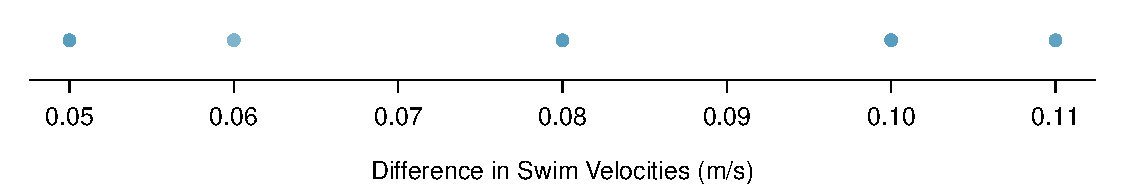
\includegraphics[width=0.9\textwidth]{ch_06a_inference_for_means_oi_biostat/figures/swimDotPlot/swimDotPlot}
	\caption{A dot plot of differences in swim velocities.}
	\label{swimDotPlot}
\end{figure}

Let $\overline{x}_{\text{diff}}$ denote the sample average of the differences in maximum velocity, $s_{\text{diff}}$ the sample standard deviation of the differences, and $n$ the number of pairs in the dataset. The $t$-statistic used to test $H_0$ vs. $H_A$ is:
\[\frac{\overline{x}_{\text{diff}} - \delta_0} {s_{\text{diff}}/\sqrt{n}},\]
where in this case $\delta_0 = 0$.\footnote{This value is specified by the null hypothesis of no difference.}

\begin{examplewrap}
\begin{nexample}{Using the data in Figure~\ref{swimSuitTimes}, conduct a two-sided hypothesis test at $\alpha = 0.05$ to assess whether there is evidence to suggest that wetsuits have an effect on swim velocities during a 1500m swim.}

The hypotheses are $H_0: \delta = 0$ and $H_A: \delta \neq 0$. Let $\alpha = 0.05$. 

Calculate the $t$-statistic:
\[t = \frac{\overline{x}_{\text{diff}} - \delta_0} {s_{\text{diff}}/\sqrt{n}} = \frac{0.078 - 0}{0.022/\sqrt{12}} = 12.32\]
The two-sided $p$-value is
$$ p = P(T < -\text{12.32}) + P(T > \text{12.32}), $$
where $t$ has a $t$-distribution with $n-1 = 11$  degrees of freedom.
The $t$-table shows that $p < 0.01$. Software can be used to show that $p = 2.3 \times 10^{-7}$, a very small value indeed.  
	
The data support the claim that the wetsuits changed swim velocity in a 1500m swim. The observed average increase of 0.078~m/s is significantly different than the null hypothesis of no change, and suggests that swim velocities are higher when swimmers wear wetsuits as opposed to swimsuits.	
\end{nexample}
\end{examplewrap}

\index{t-test!paired data|)}

Calculating confidence intervals for paired data is also based on the differences between the values in each pair; the same approach as for single-sample data can be applied on the differences. For example, a two-sided 95\% confidence interval for paired data has the form:
\[ \left(
  \overline{x}_{\text{diff}} - t^\star_{df} \times \frac{s_{\text{diff}}}{\sqrt{n}},
  \:\: \overline{x}_{\text{diff}} + t^\star_{df} \times \frac{s_{\text{diff}}}{\sqrt{n}} \right), 
\]
where $t^\star$ is the point on a $t$-distribution with $df = n - 1$ for $n$ pairs, with area 0.025 to its right.

%\textD{\newpage}

\begin{exercisewrap}
\begin{nexercise} 
Using the data in Figure~\ref{swimSuitTimes}, calculate a 95\% confidence interval for the average difference in swim velocities during a 1500m swim. Is the interval consistent with the results of the hypothesis test?\footnotemark{}
\end{nexercise}
\end{exercisewrap}
\footnotetext{Use the values of $\overline{x}_{\text{diff}}$ and $s_{\text{diff}}$ as calculated previously: 0.078 and 0.022. The $t^\star$ value of 2.20 has $df = 11$ and 0.025 area to the right. The confidence interval is ($0.078 \pm \frac{0.022}{\sqrt{12}}$) $\to$ (0.064, 0.091) m/s. With 95\% confidence, $\delta$ lies between 0.064 m/s and 0.09 m/s. The interval does not include 0 (no change), which is consistent with the result of the hypothesis test.}

The general approach when analyzing paired data is to first calculate the differences between the values in each pair, then use those differences in methods for confidence intervals and tests for a single sample.  Any conclusion from an analysis should be stated in terms of the original paired measurements.

%%% CAMBIO: Seccion anyadida


\section{Testing the equality of two variances}
\label{TwoVariancesSection}
The difference of the variances between two groups is frequently used to study
the quality of two different procedures or treatment. Less variability
is associated to greater quality. For this course, another use is to confirm that the variances of a continuous variable for two groups are identical. This is going to be a previous step before studying hypothesis testing of the mean of independent sample. Later, we are going to distinguish between two-sample test for independent data with non-identical variances (\ref{differenceOfTwoMeansEqualVar}) and with identical variances (\ref{differenceOfTwoMeans}).



Given two normally distributed  random variables, two sample are extracted.  Let  $s_1^2$ be the variance of a sample with $n_1$ following a normal distribution mean $\mu_1$ and standard deviation $\sigma_1$ and let $s_2^2$  be the variance of a sample with $n_2$ following a normal distribution mean $\mu_2$ and standard deviation $\sigma_2$.  The quotient 
$$F=\frac{s_1^2/\sigma_1^2}{s_2^2/\sigma_2^2}$$ 
follows a distribution called Snedecor's F distribution with a numerator with degree of freedom $n_1-1$ and a denominator with degree of freedom $n_2-1$. In the Figure~\ref{SnedecorFdist} several probability densitity function are displayed.

A table with 95 and 97.5 percentiles of the Snedecor's F distribution can be found on the Appendix~B.  The 5 and 2.5 percentiles can be found by means of the following formula, based on interchanging the roles of the numerator and denominator:

$$
F_{n_1,n_2,\alpha }=\frac{1}{F_{n_2,n_1,1-\alpha}} 
$$
%Citar correctamente cuando sea posible. 



\begin{figure}[h]
	\centering
	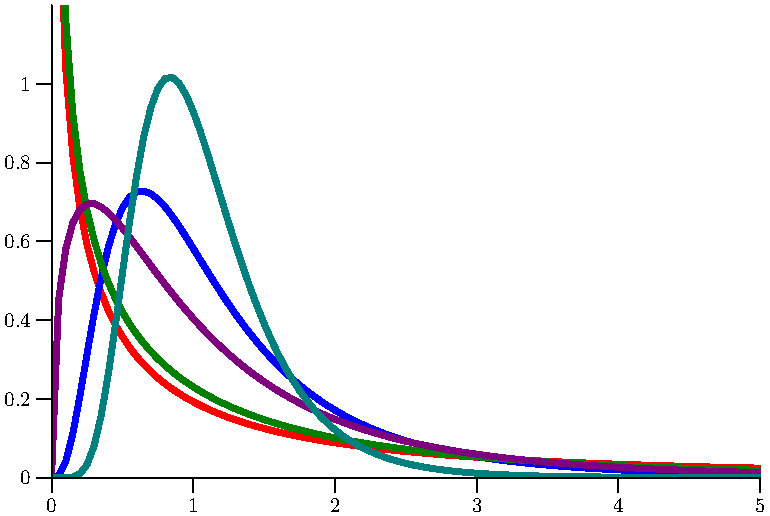
\includegraphics[width=0.58\textwidth]{ch_06a_inference_for_means_oi_biostat/figures/FDist/Snedecor-0}
	\caption{Snedecor's F distributions. Several probability density functions are displayed. The red curve corresponds to degree of freedom 1 in the numerator and 2 in the denominator.  The blue curve corresponds to degree of freedom 9 in the numerator and 9 in the denominator.  The red curve corresponds to degree of freedom 1 in the numerator and 2 in the denominator.  The green curve corresponds to degree of freedom 1 in the numerator and 10 in the denominator.  The dark green curve corresponds to degree of freedom 20 in the numerator and 25 in the denominator.}
	\label{SnedecorFdist}
      \end{figure}
      
\begin{examplewrap}
  \begin{nexample}{
The time of a surgical  intervention in horses using two different
techniques is being estimated to improve the quality of the treatment. It's assume that the time of surgical intervention is a
normal distribution for both of the techniques.  The sample variance
is $s_1=50$ for 31 horses which technique was 1 and $s_2=24$ for 25
horses operated with the technique 2. Test whether the variance of
these variable is significantly different. 
}

The null--hypothesis is 
\begin{align*}
H_0: &   \sigma_A=\sigma_B & H_A:&\sigma_A\neq\sigma_B
\end{align*}
 and 
    the sample size are $n_A=31$ and $n_B=25$, and the variances
    $s^2_A=50$ and $s^2_B=24$.

The test statistics is $F=s^2_A/s^2_B=50/24= 2.08$ 

The acceptance region is
$(F_{30,24,.025},F_{30,24,.975})=(\frac{1}{F_{24,30,.975}},F_{30,24,.975})=(\frac{1}{2.1359},2.2090)=(0.4681,2.2090)$.
 
The value of the test statistic is inside a acceptance region and the
null hypothesis is failed to reject. The study does not provide enough evidence to say that the two groups have different variances.  

\end{nexample}
\end{examplewrap}
% __________________


\section[Two-sample test for independent data with identical variances]{Two-sample test for independent data (identical variances)}
\label{differenceOfTwoMeansEqualVar}


In this section we consider a difference in two population means, $\mu_1 - \mu_2$, under the condition that the data are not paired. If the data are not paired and there is not a natural link between the individuals in the two groups, it is said to be \term{independent samples}. In this section, the variances are assumed to be identical. This assumption can be considered reasonable if we fail to reject the null hypothesis of the test of two variances, which we have studied on the previous section. When variances cannot be assumed identical, the test statistic is different and it will be studied on the next section.  The paired and independent samples methods are similar in theory but different in the details. Just as with a single sample, we identify conditions to ensure a point estimate of the difference $\bar{x}_1 - \bar{x}_2$ is nearly normal. Next we introduce a formula for the standard error. 

%__________________

\subsection{Pooled standard deviation estimate (if variances are identical for both groups)}
\label{pooledStandardDeviations}

Occasionally, two populations will have standard deviations that are so similar that they can be treated as identical. For example, historical data or a well-understood biological mechanism may justify this strong assumption. In such cases, we can make our $t$ distribution approach slightly more precise by using a pooled standard deviation.

The \term{pooled standard deviation} of two groups is a way to use data from both samples to better estimate the standard deviation and standard error. If $s_1^{}$ and $s_2^{}$ are the standard deviations of groups 1 and 2 and there are good reasons to believe that the population standard deviations are equal, then we can obtain an improved estimate of the group variances by pooling their data:
\begin{align*}
s_{pooled}^2 = \frac{s_1^2\times (n_1-1) + s_2^2\times (n_2-1)}{n_1 + n_2 - 2}
\end{align*}
where $n_1$ and $n_2$ are the sample sizes, as before. To use this new statistic, we substitute $s_{pooled}^2$ in place of $s_1^2$ and $s_2^2$ in the standard error formula, and we use an updated formula for the degrees of freedom:
\begin{align*}
df = n_1 + n_2 - 2
\end{align*}

The benefits of pooling the standard deviation are realized through obtaining a better estimate of the standard deviation for each group and using a larger degrees of freedom parameter for the $t$ distribution. Both of these changes may permit a more accurate model of the sampling distribution of $\bar{x}_1 - \bar{x}_2$.

%\begin{caution}
{Pooling standard deviations should be done only after careful research}
{A pooled standard deviation is only appropriate when background research indicates the population standard deviations are nearly equal. When the sample size is large and the condition may be adequately checked with data, the benefits of pooling the standard deviations greatly diminishes.}
%\end{caution}

\subsection{Hypothesis testing with equal variance} 
\label{NTequalV}
   Assume that the variances $\sigma_1^2 = \sigma_2^2 = \sigma^2$ are equal but
unknown in both groups.  The sample pool variance is considered the point estimate of the variance for both groups. Therefore, the standard error is the  pool standard error  multiplied by the square root of $1/n_1$ plux $1/n_2$. 

In order to test whether the mean population are identical in both groups, the following t statistic is defined 
 $$ t=
  \frac{(\overline{x}_1-\overline{x}_2)}
  {S_p\sqrt{\frac{1}{n_1}+\frac{1}{n_2}}}.
  $$  
If the mean population are equal in both group, this test statistic
follows a Student's t distibution with degree of freedom $n_1+n_2-2$. 

\begin{examplewrap}
\begin{nexample}{
 Two simple random samples are selected from the adult male population of Beijing
  and Shanghai, respectively. The variable height (cm) of the individuals in each
  sample has the following data: \newline 
  %\begin{center}
  \begin{tabular}{l|l|l|l}
    Beijing & $n_B=10$ & $\overline{x}_B=169$ & $s_B^2=1\,800$ \\
  \hline  Shanghai & $n_S=21$ & $\overline{x}_S=171$ & $s_S^2=1\,400$ \\
  \end{tabular}  
  % \end{center}
  \newline
Is there a significant difference between the height of male
population?
}
First, test whether the groups have identical variance $\sigma_B=\sigma_S$:\\
The statistic  $F=\frac{1800}{1400}=1.2857$ and the  
 acceptance region with numeratos 10 and 21  is  $(F_{9,20,.025},F_{9,20,.975})=(0.27,2.84) $
Therefore, it is  failed to reject that the variances are different. Let us assume that
the variances are identical.  
  
Second, test if the mean are identical in both groups. 

The pooled variance ($s^2_{\mbox{pooled}}$) in this case is 
$$S_{\mbox{pooled}}^2 = \frac{(n_B-1)S_B^2+(n_S-1)S_S^2}{n_B+n_S-2}= \frac{9\cdot
  1800+20\cdot 1400}{29}=1524.138$$
The test statistic is 
$$
t=
\frac{(\overline{x}_B-\overline{x}_S)}
  {S_p\sqrt{\frac{1}{n_B}+\frac{1}{n_S}}}
=\frac{169-171}{\sqrt{1524.138}\sqrt{\frac{1}{10}+\frac{1}{21}}}=-0.1333358
$$  

The acceptance region is
$(-t_{29,.975},t_{29,.975})=(-2.04523,2.04523)$.

We fail to reject the null hypothesis. The difference between the
adult male people in both city is not
statistically significant.  
\end{nexample}
\end{examplewrap}
\section[Two-sample test for independent data with non-identical variances]{Two-sample test for independent data (non-identical variances)}
\label{differenceOfTwoMeans}

In this section, we study the situation when identical variances cannot be assumed. 

Does treatment using embryonic stem cells (ESCs) help improve heart function following a heart attack? New and potentially risky treatments are sometimes tested in animals before studies in humans are conducted.  In a 2005 paper in \textit{Lancet}, Menard, et al. describe an experiment in which 18 sheep with induced heart attacks were randomly assigned to receive cell transplants containing either ESCs or inert material.\footnote{Menard C, et al., Transplantation of cardiac-committed mouse embryonic stem cells to infarcted sheep myocardium: a preclinical 2005; 366:1005-12, doi \url{https://doi.org/10.1016/S0140-6736(05)67380-1}}  Various measures of cardiac function were measured 1 month after the transplant.

This design is typical of an intervention study. The analysis of such an experiment is an example of drawing inference about the difference in two population means, $\mu_1 - \mu_2$, when the data are independent, i.e., not paired. The point estimate of the difference, $\overline{x}_1 - \overline{x}_2$, is used to calculate a $t$-statistic that is the basis of confidence intervals and tests.


\subsection{Confidence interval for a difference of means}
\label{confidenceIntervalDifferenceMeans}

\index{data!stem cells, heart function|(}
\index{point estimate!difference of two means|(}
Figure~\ref{summaryStatsForSheepHeartDataWhoReceivedMiceESCs} contains summary statistics for the 18 sheep.\footnote{The data are accessible as the dataset \data{stem.cells} in the \texttt{openintro} \textsf{R} package.}  Percent change in heart pumping capacity was measured for each sheep. A positive value corresponds to increased pumping capacity, which generally suggests a stronger recovery from the heart attack.  Is there evidence for a potential treatment effect of administering stem cells?


\begin{figure}[h]
\centering
\begin{tabular}{l rrrrr}
\hline
\hspace{10mm}	& $n$	& $\overline{x}$	& $s$  	 \\
\hline
ESCs		& 9		& 3.50		& 5.17  	\\
control		& 9		& -4.33		& 2.76  	 \\
\hline
\end{tabular}
\caption{Summary statistics of the embryonic stem cell study.}
\label{summaryStatsForSheepHeartDataWhoReceivedMiceESCs}
\end{figure}

%\textD{\newpage}

\begin{figure}[h]
	\centering
	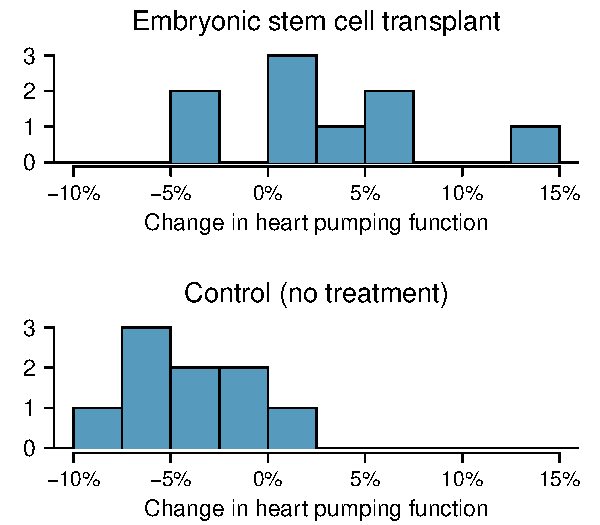
\includegraphics[width=0.58\textwidth]{ch_06a_inference_for_means_oi_biostat/figures/stemCellTherapyForHearts/stemCellTherapyForHearts}
	\caption{Histograms for both the embryonic stem cell group and the control group. Higher values are associated with greater improvement.}
	\label{stemCellTherapyForHearts}
\end{figure}

Figure~\ref{stemCellTherapyForHearts} shows that the distributions of percent change do not have any prominent outliers, which would indicate a deviation from normality; this suggests that each sample mean can be modeled using a $t$-distribution. Additionally, the sheep in the study are independent of each other, and the sheep between groups are also independent. Thus, the $t$-distribution can be used to model the difference of the two sample means.

\begin{onebox}{Using the $\pmb{\MakeLowercase{t}}$-distribution for a difference in means}
\label{ConditionsForTwoSampleTDist}The $t$-distribution can be used for inference when working with the standardized difference of two means if (1) each sample meets the conditions for using the $t$-distribution and (2) the samples are independent.
\end{onebox}

\index{point estimate!difference of two means|)}
\index{confidence interval!difference of two means|(}

A confidence interval for a difference of two means has the same basic structure as previously discussed confidence intervals:

\[(\overline{x}_{1} - \overline{x}_{2}) \pm t^\star_{df} \times \text{ SE }. \]

\index{standard error (SE)!difference in means}

The following formula is used to calculate the standard error of $\overline{x}_{1} - \overline{x}_{2}$. Since $\sigma$ is typically unknown, the standard error is estimated by using $s$ in place of $\sigma$. 

\[
SE_{\overline{x}_{1} - \overline{x}_{2}} = \sqrt{\frac{\sigma_{1}^2}{n_{1}} + \frac{\sigma_{2}^2}{n_{2}}} \approx \sqrt{\frac{s_{1}^2}{n_{1}} + \frac{s_{2}^2}{n_{2}}}.
\]

In this setting, the $t$-distribution has a somewhat complicated formula for the degrees of freedom that is usually calculated with software.\footnote{See Section~\ref{inferenceForNumericalDataNotes} for the formula.} An alternative approach uses the smaller of $n_1 - 1$ and $n_2 - 1$ as the degrees of freedom.\footnote{This technique for degrees of freedom is conservative with respect to a Type~1 Error; it is more difficult to reject the null hypothesis using this approach for degrees of freedom.}

%\textD{\newpage}

\begin{onebox}{Distribution of a difference of sample means}
The sample difference of two means, $\overline{x}_1 - \overline{x}_2$, can be modeled using the $t$-distribution and the standard error
\begin{eqnarray}
\textstyle
SE_{\overline{x}_{1} - \overline{x}_{2}} = \sqrt{\frac{s_1^2}{n_1} + \frac{s_2^2}{n_2}}
\label{seOfDifferenceInMeans}
\end{eqnarray}
when each sample mean can itself be modeled using a $t$-distribution and the samples are independent. To calculate the degrees of freedom without using software, use the smaller of $n_1 - 1$ and $n_2 - 1$.
\end{onebox}

\begin{examplewrap}
\begin{nexample}{Calculate and interpret a 95\% confidence interval for the effect of ESCs on the change in heart pumping capacity of sheep following a heart attack.}
	
The point estimate for the difference is $\overline{x}_1 - \overline{x}_2 = \overline{x}_{\text{esc}} - \overline{x}_{\text{control}} = 7.83$.	
	
The standard error is:	
\[\sqrt{\frac{s_{1}^2}{n_{1}} + \frac{s_{2}^2}{n_{2}}} = \sqrt{\frac{5.17^2}{9} + \frac{2.76^2}{9}} = 1.95.\]
	
Since $n_1 = n_2 = 9$, use $df = 8$; $t^{\star}_{8} = 2.31$ for a 95\% confidence interval. Alternatively, computer software can provide more accurate values: $df = 12.225, t^\star = 2.174$.

The confidence interval is given by:
\[(\overline{x}_{1} - \overline{x}_{2}) \pm t^\star_{df} \times \text{ SE } \quad\rightarrow\quad
7.83 \ \pm\ 2.31\times 1.95 \quad\rightarrow\quad (3.38, 12.38). \]

With 95\% confidence, the average amount that ESCs improve heart pumping capacity lies between 3.38\% to 12.38\%.\footnotemark{} The data provide evidence for a treatment effect of administering stem cells.
\end{nexample}
\end{examplewrap}
\footnotetext{From software, the confidence interval is (3.58, 12.08).}

\index{data!stem cells, heart function|)}
\index{confidence interval!difference of two means|)}

\subsection{Hypothesis tests for a difference in means}
\label{testingDifferenceMeans}


\index{t-test!two independent groups|(}

\index{data!births|(}

Is there evidence that newborns from mothers who smoke have a different average birth weight than newborns from mothers who do not smoke? The dataset \data{births} contains data from a random sample of 150 cases of mothers and their newborns in North Carolina over a year; there are 50 cases in the smoking group and 100 cases in the nonsmoking group.\footnote{This dataset is available in the \texttt{openintro} \textsf{R} package. }

\begin{figure}[h]
\centering
\begin{tabular}{rrrrrll}
  \hline
 & fAge & mAge & weeks & weight & sexBaby & smoke \\ 
  \hline
1 & NA & 13 &  37 & 5.00 & female & nonsmoker \\ 
  2 & NA & 14 &  36 & 5.88 & female & nonsmoker \\ 
  3 & 19 & 15 &  41 & 8.13 & male & smoker \\ 
  $\vdots$ &   $\vdots$ &   $\vdots$ &   $\vdots$ &   $\vdots$ &   $\vdots$ \\
  150 & 45 & 50 &  36 & 9.25 & female & nonsmoker \\ 
   \hline
\end{tabular}
\caption{Four cases from the \data{births} dataset.}
\label{babySmokeDF}
\end{figure}

%\textD{\newpage}

\begin{examplewrap}
\begin{nexample} {Evaluate whether it is appropriate to apply the $t$-distribution to the difference in sample means between the two groups.}
Since the data come from a simple random sample and consist of less than 10\% of all such cases, the observations are independent. While each distribution is strongly skewed, the large sample sizes of 50 and 100 allow for the use of the $t$-distribution to model each mean separately. Thus, the difference in sample means may be modeled using a $t$-distribution.	
\end{nexample}
\end{examplewrap}

\begin{figure}[hhh]
\centering
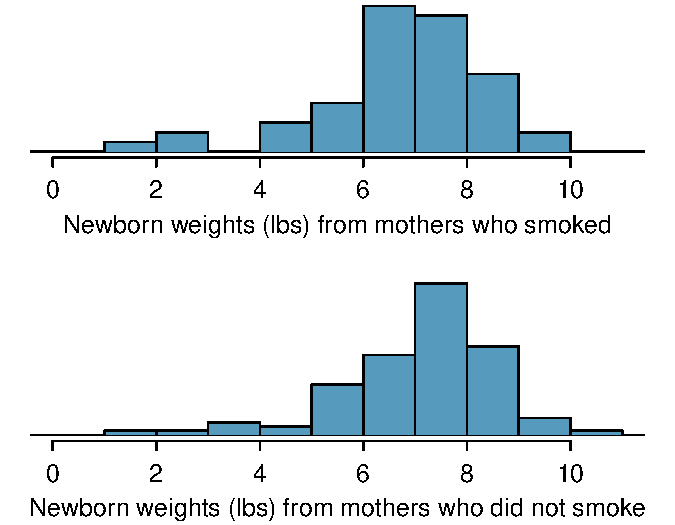
\includegraphics[width=0.63\textwidth]{ch_06a_inference_for_means_oi_biostat/figures/babySmokePlotOfTwoGroupsToExamineSkew/babySmokePlotOfTwoGroupsToExamineSkew}
\caption{The top panel represents birth weights for infants whose mothers smoked. The bottom panel represents the birth weights for infants whose mothers who did not smoke. The distributions exhibit moderate-to-strong and strong~skew, respectively.\index{skew!example: strong}}
\label{babySmokePlotOfTwoGroupsToExamineSkew}
\end{figure}

A hypothesis test can be conducted to evaluate whether there is a relationship between mother's smoking status and average newborn birth weight. The null hypothesis represents the case of no difference between the groups, $H_0: \mu_{ns} - \mu_{s} = 0$, where $\mu_{ns}$ represents the population mean of newborn birthweight for infants with mothers who did not smoke, and $\mu_s$ represents mean newborn birthweight for infants with mothers who smoked. Under the alternative hypothesis, there is some difference in average newborn birth weight between the groups, $H_A: \mu_{ns} - \mu_{s} \neq 0$. The hypotheses can also be written as $H_0: \mu_{ns} = \mu_{s}$ and $H_A: \mu_{ns} \neq \mu_{s}$.

\begin{onebox}{Stating hypotheses for two-group data}
When testing a hypothesis about two independent groups, directly compare the two population means and state hypotheses in terms of $\mu_1$ and $\mu_2$.
\begin{itemize}
	\item For a two-sided test, $H_0: \mu_{1} = \mu_{2}$; $H_A: \mu_{1} \neq \mu_{2}$.
	\item For a one-sided test, either $H_0: \mu_{1} = \mu_{2}$; $H_A: \mu_{1} > \mu_{2}$ or  $H_0: \mu_{1} = \mu_{2}$; $H_A: \mu_{1} < \mu_{2}$.
\end{itemize}
\end{onebox}


%\textD{\newpage}

In this setting, the formula for a $t$-statistic is:
\[
t = \dfrac{(\overline{x}_1 - \overline{x}_2) - (\mu_1 - \mu_2)}{SE_{\overline{x}_{1} - \overline{x}_{2}}} = \dfrac{(\overline{x}_1 - \overline{x}_2) - (\mu_1 - \mu_2)}{\sqrt{\dfrac{s_{1}^{2}}{n_1} + \dfrac{s_{2}^{2}}{n_2}}}.
\]
Under the null hypothesis of no difference between the groups, $H_0: \mu_{1} - \mu_{2} = 0$, the formula simplifies to
\[t = \dfrac{(\overline{x}_1 - \overline{x}_2)}{\sqrt{\dfrac{s_{1}^{2}}{n_1} + \dfrac{s_{2}^{2}}{n_2}}}.\]

\begin{examplewrap}
\begin{nexample}{Using Figure~\ref{summaryStatsBabySmoke}, conduct a hypothesis test to evaluate whether there is evidence that newborns from mothers who smoke have a different average birth weight than newborns from mothers who do not smoke.}

The hypotheses are $H_0: \mu_{1} = \mu_{2}$ and $H_A: \mu_{1} \neq \mu_{2}$, where $\mu_{1}$ represents the average newborn birth weight for nonsmoking mothers and $\mu_{2}$ represents average newborn birth weight for mothers who smoke. Let $\alpha = 0.05$. 	

Calculate the $t$-statistic:

\[t = \dfrac{(\overline{x}_1 - \overline{x}_2)}{\sqrt{\dfrac{s_{1}^{2}}{n_1} + \dfrac{s_{2}^{2}}{n_2}}} = \dfrac{7.18 - 6.78}{\sqrt{\frac{1.60^2}{100} + \frac{1.43^2}{50}}} = 1.54.\]

Approximate the degrees of freedom as $50 - 1 = 49$. The $t$-score of 1.49 falls between the first and second columns in the $df = 49$ row of the $t$-table, so the two-sided $p$-value is between 0.10 and 0.20.\footnotemark{}

This $p$-value is larger than the significance value, 0.05, so the null hypothesis is not rejected. There is insufficient evidence to state there is a difference in average birth weight of newborns from North Carolina mothers who did smoke during pregnancy and newborns from North Carolina mothers who did not smoke during pregnancy.
\end{nexample}
\end{examplewrap}
\footnotetext{From \textsf{R}, $df = 89.277$ and $p = 0.138$.}

\begin{figure}[hhh]
	\centering
	\begin{tabular}{lrr}
		& smoker & nonsmoker \\
		\hline
		mean & 6.78 & 7.18 \\
		st. dev. & 1.43 & 1.60 \\
		samp. size & 50 & 100 \\
		\hline
	\end{tabular}
	\caption{Summary statistics for the \data{births} dataset.}
	\label{summaryStatsBabySmoke}
\end{figure}		

\index{data!births|)}

\index{t-test!two independent groups|)}


%\textD{\newpage}


\subsection{The paired test vs. independent group test}
\label{pairedVsTwoGroups}

In the two-sample setting, students often find it difficult to determine whether a paired test or an independent group test should be used.  The paired test applies only in situations where there is a natural pairing of observations between groups, such as in the \data{swim} data. Pairing can be obvious, such as the two measurements for each swimmer, or more subtle, such as measurements of respiratory function in twins, where one member of the twin pair is treated with an experimental treatment and the other with a control. In the case of two independent groups, there is no natural way to pair observations.

A common error is to overlook pairing in data and assume that two groups are independent. The swimsuit data can be used to illustrate the possible harm in conducting an independent group test rather than a paired test. In Section~\ref{pairedData}, the paired $t$-test showed a significant difference in the swim velocities between swimmers wearing wetsuits versus regular swimsuits. Suppose the analysis had been conducted without accounting for the fact that the measurements were paired.

The mean and standard deviation for the 12 wet suit velocities are 1.51 and 0.14 (m/sec), respectively, and 1.43 and 0.14 (m/sec) for the 12 swim suit velocities. A two-group test statistic is:
\[t = \frac{1.52 - 1.43}{\sqrt{0.14^2/12 + 0.14^2/12}} = 1.37. \]
If the degrees of freedom are approximated as $11 = 12 - 1$, the two-sided $p$-value as calculated from software is 0.20. According to this method, the null hypothesis of equal mean velocities for the two suit types would not be rejected.

It is not difficult to show that the numerator of the paired test (the average of the within swimmer differences) and the numerator of the two-group test (the difference of the average times for the two groups) are identical. The values of the test statistics differ because the denominators are different\textemdash specifically, the standard errors associated with each statistic are different.  For the paired test statistic, the standard error uses the standard deviation of the within pair differences (0.22) and has value $0.022/\sqrt{12} = 0.006$. The two-group test statistic combines the standard deviations for the original measurements and has value $\sqrt{0.14^2/12 + 0.14^2/12} = 0.06$.  The standard error for the two-group test is 10-fold larger than for the paired test.  

This striking difference in the standard errors is caused by the much lower variability of the individual velocity differences compared to the variability of the original measurements. Due to the correlation between swim velocities for a single swimmer, the differences in the two velocity measurements for each swimmer are consistently small, resulting in low variability. Pairing has allowed for increased precision in estimating the difference between groups.

The swim suit data illustrates the importance of context, which distinguishes a statistical problem from a purely mathematical one. While both the paired and two-group tests are numerically feasible to calculate, without an apparent error, the context of the problem dictates that the correct approach is to use a paired test.

\begin{exercisewrap}
\begin{nexercise}
Propose an experimental design for the embryonic stem cell study in sheep that would have required analysis with a paired $t$-test.\footnotemark{}
\end{nexercise}
\end{exercisewrap}
\footnotetext{The experiment could have been done on pairs of siblings, with one assigned to the treatment group and one assigned to the control group. Alternatively, sheep could be matched up based on particular characteristics relevant to the experiment; for example, sheep could be paired based on similar weight or age. Note that in this study, a design involving two measurements taken on each sheep would be impractical.}


%\textD{\newpage}



% \subsection{Pooled standard deviation estimate}
% \label{pooledStandardDeviations}

% Occasionally, two populations will have standard deviations that are so similar that they can be treated as identical. For example, historical data or a well-understood biological mechanism may justify this strong assumption. In such cases, it can be more precise to use a pooled standard deviation to make inferences about the difference in population means.

% The \term{pooled standard deviation} of two groups uses data from both samples to estimate the common standard deviation and standard error. If there are good reasons to believe that the population standard deviations are equal, an improved estimate of the group variances can be obtained by pooling the data from the two groups:
% \begin{align*}
% s_{\text{pooled}}^2 = \frac{s_1^2 (n_1-1) + s_2^2 (n_2-1)}{n_1 + n_2 - 2},
% \end{align*}
% where $n_1$ and $n_2$ are the sample sizes, and $s_1$ and $s_2$ represent the sample standard deviations. In this setting, the $t$-statistic uses $s_{\text{pooled}}^2$ in place of $s_1^2$ and $s_2^2$ in the standard error formula, and the degrees of freedom for the $t-$statistic is the sum of the degrees of freedom for the two sample variances:
% \[
% \text{df} = (n_1 - 1) + (n_2 - 1) = n_1 + n_2 - 2.
% \]
% The $t$-statistic for testing the null hypothesis of no difference between population means becomes 
% \[
%  t = \frac{\overline{x}_1 - \overline{x}_2}{s_{\text{pooled}}\sqrt{\frac{1}{n_1} + \frac{1}{n_2}}}. 
% \]

% The formula for the two-sided confidence interval for the difference in population means is
% \[
%   (\overline{x}_1 - \overline{x}_2) \pm t^{\star} \times s_{\text{pooled}} \sqrt{\frac{1}{n_1} + \frac{1}{n_2}},
% \]
% where $t^{\star}$ is the point on a $t$-distribution with $n_1 + n_2 -2$ degrees of freedom chosen according to the confidence coefficient.

% The benefits of pooling the standard deviation are realized through obtaining a better estimate of the standard deviation for each group and using a larger degrees of freedom parameter for the $t$-distribution. Both of these changes may permit a more accurate model of the sampling distribution of $\overline{x}_1 - \overline{x}_2$, if the standard deviations of the two groups are indeed equal.  In most applications, however, it is difficult to verify the assumption of equal population standard deviations, and thus safer to use the methods discussed in Sections~\ref{confidenceIntervalDifferenceMeans} and \ref{testingDifferenceMeans}.



%__________________
% \section[Power calculations for a difference of means]{Power calculations for a difference of means}
% \label{PowerForDifferenceOfTwoMeans}

% Designing a study often involves many complex issues; perhaps the most important statistical issue in study design is the choice of an appropriate sample size. The \termsub{power}{power of a test} of a statistical test is the probability that the test will reject the null hypothesis when the alternative hypothesis is true; sample sizes are chosen to make that probability sufficiently large, typically between 80\% and 90\%. 

% Two competing considerations arise when choosing a sample size. The sample size should be sufficiently large to allow for important group differences to be detected in a hypothesis test. Practitioners often use the term `detecting a difference' to mean correctly rejecting a null hypothesis, i.e., rejecting a null hypothesis when the alternative is true. If a study is so small that detecting a statistically significant difference is unlikely even when there are potentially important differences, enrolling participants might be unethical, since subjects could potentially be exposed to a dangerous experimental treatment. However, it is also unethical to conduct studies with an overly large sample size, since more participants than necessary would be exposed to an intervention with uncertain value. Additionally, collecting data is typically expensive and time consuming; it would be a waste of valuable resources to design a study with an overly large sample size.

% This section begins by illustrating relevant concepts in the context of a hypothetical clinical trial, where the goal is to calculate a sufficient sample size for being 80\% likely to detect practically important effects.\footnote{While sample size planning is also important for observational studies, those techniques are not discussed here.} Afterwards, formulas are provided for directly calculating sample size, as well as references to software that can perform the calculations.


% \subsection{Reviewing the concepts of a test}

% \begin{examplewrap}
% \begin{nexample}{A company would like to run a clinical trial with participants whose systolic blood pressures are between 140 and 180 mmHg. Suppose previously published studies suggest that the standard deviation of patient blood pressures will be about 12 mmHg, with an approximately symmetric distribution.\footnotemark{} What would be the approximate standard error for $\overline{x}_{ \text{trmt}} - \overline{x}_{ \text{ctrl}}$ if 100 participants were enrolled in each treatment group?}
% The standard error is calculated as follows:
% \begin{align*}
% SE_{\overline{x}_{ \text{trmt}} - \overline{x}_{ \text{ctrl}}}
%   = \sqrt{\frac{s_{ \text{trmt}}^2}{n_{ \text{trmt}}} + \frac{s_{ \text{ctrl}}^2}{n_{ \text{ctrl}}}}
%   = \sqrt{\frac{12^2}{100} + \frac{12^2}{100}}
%   = 1.70.
% \end{align*}
% This may be an imperfect estimate of $SE_{\overline{x}_{ \text{trmt}} - \overline{x}_{\text{ctrl}}}$, since the standard deviation estimate of 12 mmHg from prior data may not be correct. However, it is sufficient for getting started, and making an assumption like this is often the only available option. 
% \end{nexample}
% \end{examplewrap}
% \footnotetext{In many studies like this one, each participant's blood pressure would be measured at the beginning and end of the study, and the outcome measurement for the study would be the average difference in blood pressure in each of the treatment groups. For this hypothetical study, we assume for simplicity that blood pressure is measured at only the end of the study, and that the randomization ensures that blood pressures at the beginning of the study are equal (on average) between the two groups.}

% %\textD{\newpage}

% Since the degrees of freedom are greater than 30, the distribution of $\overline{x}_{ \text{trmt}} - \overline{x}_{ \text{ctrl}}$ will be approximately normal. Under the null hypothesis, the mean is 0 and the standard deviation is 1.70 (from the standard error).

% \begin{figure}[h]
% 	\centering
% 	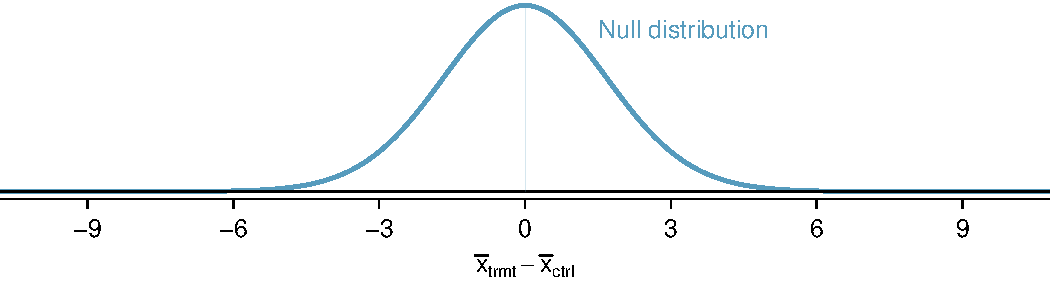
\includegraphics[width=0.85\textwidth]{ch_inference_for_means_oi_biostat/figures/power_null_0_1-7/power_null_A_0_1-7}
% 	\caption{Null distribution for the t-statistic in Example~\ref{example-power_null_A_0_1-7}.}
% 	\label{power_null_A_0_1-7}
% \end{figure}

% \begin{examplewrap}
% \begin{nexample}{For what values of $\overline{x}_{\text{trmt}} - \overline{x}_{\text{ctrl}}$ would the null hypothesis be rejected, using $\alpha = 0.05$?}%
% \label{example-power_null_A_0_1-7}%
% If the observed difference is in the far left or far right tail of the null distribution, there is sufficient evidence to reject the null hypothesis.
% For $\alpha = 0.05$, $H_0$ is rejected if the difference is in the lower 2.5\% or upper 2.5\% tail:
% \begin{description}
% \setlength{\itemsep}{0mm}
% \item[Lower 2.5\%:] For the normal model, this is 1.96 standard errors below 0, so any difference smaller than $-1.96 \times 1.70 = -3.332$~mmHg.
% \item[Upper 2.5\%:] For the normal model, this is 1.96 standard errors above 0, so any difference larger than $1.96 \times 1.70 = 3.332$~mmHg.
% \end{description}
% The boundaries of these \termsub{rejection regions}{rejection region} are shown below. Note that if the new treatment is effective, mean blood pressure should be lower in the treatment group than in the control group; i.e., the difference should be in the lower tail.
% \begin{center}
% 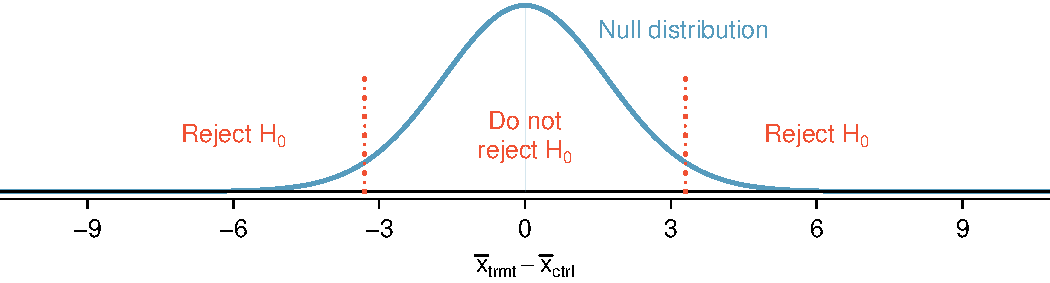
\includegraphics[width=0.85\textwidth]{ch_inference_for_means_oi_biostat/figures/power_null_0_1-7/power_null_B_0_1-7_with_rejection_region}
% \end{center}
% \end{nexample}
% \end{examplewrap}

% The next step is to perform some hypothetical calculations to determine the probability of rejecting the null hypothesis if the alternative hypothesis were true.


% %\textD{\newpage}


% \subsection{Computing the power for a 2-sample test}

% If there is a real effect from an intervention, and the effect is large enough to have practical value, the probability of detecting that effect is referred to as the \termsub{power}{power of a test}. Power can be computed for different sample sizes or different effect sizes. 

% There is no easy way to define when an effect size is large enough to be of value; this is not a statistical issue. For example, in a clinical trial, the scientifically significant effect is the incremental value of the intervention that would justify changing current clinical recommendations from an existing intervention to a new one. In such a setting, the effect size is usually determined from long discussions between the research team and study sponsors. 

% Suppose that for this hypothetical blood pressure medication study, the researchers are interested in detecting any effect on blood pressure that is 3 mmHg or larger than the standard medication. Here, 3 mmHg is the minimum \term{population effect size} of interest. 

% \begin{examplewrap}
% \begin{nexample}{Suppose the study proceeded with 100 patients per treatment group and the new drug does reduce average blood pressure by an additional 3~mmHg relative to the standard medication. What is the probability of detecting this effect?}\label{PowerFor100AtNeg3}%
% Determine the sampling distribution for $\overline{x}_{\text{trmt}} - \overline{x}_{\text{ctrl}}$ when the true difference is $-3$~mmHg; this has the same standard deviation of 1.70 as the null distribution, but the mean is shifted 3 units to the left. Then, calculate the fraction of the distribution for $\overline{x}_{\text{trmt}} - \overline{x}_{\text{ctrl}}$ that falls within the rejection region for the null distribution, as shown in Figure~\ref{power_null_D_0_1-7_with_alt_at_3_and_shaded}.

% The probability of being in the left side of the rejection region ($x < -3.332$) can be calculated by converting to a $Z$-score and using either the normal probability table or statistical software.\footnotemark{}

% \[
% 	Z = \frac{-3.332 - (-3)}{1.7}= -0.20 \quad \to \quad P(Z \leq -0.20) = 0.4207.
% \]

% The power for the test is about 42\% when $\mu_{\text{trmt}} - \mu_{\text{ctrl}} = -3$~mm/Hg and each group has a sample size of 100.
% \end{nexample}
% \end{examplewrap}
% \footnotetext{The probability of being in the right side of the rejection region is negligible and can be ignored.}

% \begin{figure}[h]
% \begin{center}
% 	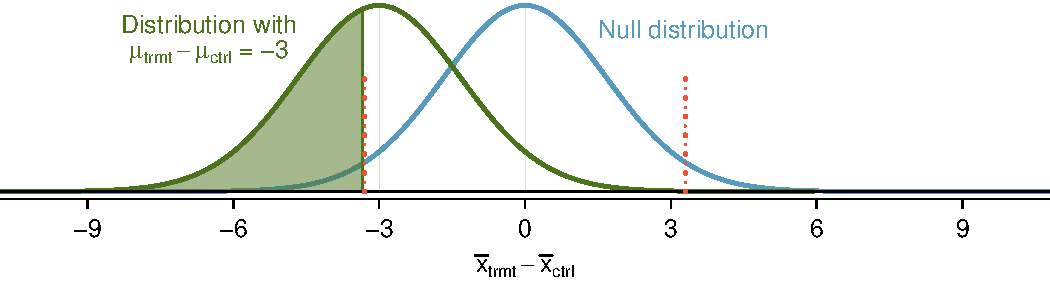
\includegraphics[width=0.87\textwidth]{ch_inference_for_means_oi_biostat/figures/power_null_0_1-7/power_null_D_0_1-7_with_alt_at_3_and_shaded}
% 	\caption{The rejection regions are outside of the dotted lines. Recall that the boundaries for $\alpha = 0.05$ were calculated to be $\pm 3.332$ mmHg.}
% 	\label{power_null_D_0_1-7_with_alt_at_3_and_shaded}
% \end{center}	
% \end{figure}


% %\textD{\newpage}


% \subsection{Determining a proper sample size}

% The last example demonstrated that with a sample size of 100 in each group, there is a probability of about 0.42 of detecting an effect size of 3~mmHg. If the study were conducted with this sample size, even if the new medication reduced blood pressure by 3~mmHg compared to the control group, there is a less than 50\% chance of concluding that the medication is beneficial. Studies with low power are often inconclusive, and there are important reasons to avoid such a situation:

% \begin{itemize}
% 	\setlength{\itemsep}{0mm}
% 	\item Participants were subjected to a drug for a study that may have little scientific value. 
	
% 	\item The company may have invested hundreds of millions of dollars in developing the new drug, and may now be left with uncertainty about its potential. 
	
% 	\item Another clinical trial may need to be conducted to obtain a more conclusive answer as to whether the drug does hold any practical value, and that would require substantial time and expense. 
% \end{itemize}

% To ensure a higher probability of detecting a clinically important effect, a larger sample size should be chosen. What about a study with 500 patients per group?

% \begin{exercisewrap}
% \begin{nexercise}
% Calculate the power to detect a change of -3~mmHg  using a sample size of 500 per group. Recall that the standard deviation of patient blood pressures was expected to be about 12 mmHg.\footnotemark{}
% \begin{enumerate}[(a)]
% \setlength{\itemsep}{0mm}
% \item Determine the standard error.
% \item Identify the null distribution and rejection regions, as well as the alternative distribution when $\mu_{trmt} - \mu_{ctrl} = -3$.
% \item Compute the probability of rejecting the null hypothesis.
% \end{enumerate}
% \end{nexercise}
% \end{exercisewrap}
% \footnotetext{(a) The standard error will now be $SE = \sqrt{\frac{12^2}{500} + \frac{12^2}{500}} = 0.76$.\\
% (b) The null distribution, rejection boundaries, and alternative distribution are shown below. The rejection regions are the areas outside the two dotted lines at $\overline{x}_{trmt} - \overline{x}_{ctrl} \pm 0.76 \times 1.96 = \pm 1.49$. \\
% 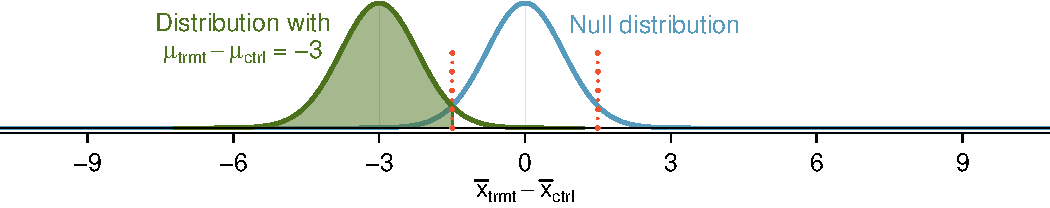
\includegraphics[width=0.8\textwidth]{ch_inference_for_means_oi_biostat/figures/power_null_0_0-76/power_null_0_0-76_with_alt_at_3_and_shaded} \\
% (c) Compute the $Z$-score and find the tail area, $Z = \frac{-1.49 - (-3)}{0.76} = 1.99 \to P(Z \leq 1.99) = 0.9767$, which is the power of the test for a difference of 3 mmHg. With 500 patients per group, the study would be 97.7\% likely to detect an effect size of 3~mmHg.}

% With a sample size of 500 per group, the power of the test is much larger than necessary. Not only does this lead to a study that would be overly expensive and time consuming, it also exposes more patients than necessary to the experimental drug. 

% Sample sizes are generally chosen such that power is around 80\%, although in some cases 90\% is the target. Other values may be reasonable for a specific context, but 80\% and 90\% are most commonly chosen as a good balance between high power and limiting the number of patients exposed to a new treatment (as well as reducing experimental costs). 

% %\textD{\newpage}

% \begin{examplewrap}
% \begin{nexample}{Identify the sample size that would lead to a power of 80\%.}

% The $Z$-score that defines a lower tail area of 0.80 is about $Z = 0.84$. In other words, 0.84 standard errors from -3, the mean of the alternative distribution. 

% \begin{center}
% 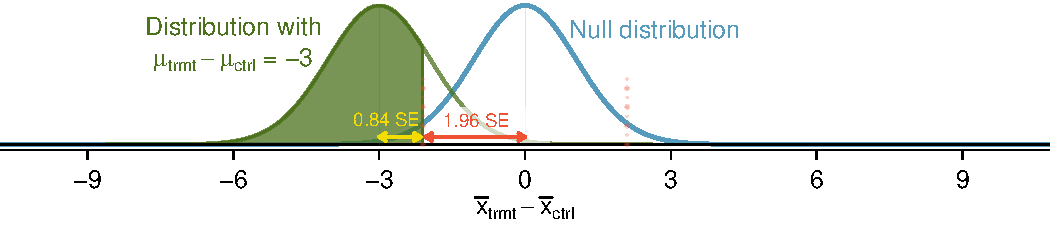
\includegraphics[width=0.93\textwidth]{ch_inference_for_means_oi_biostat/figures/power_best_sample_size/power_best_sample_size}
% \end{center}

% For $\alpha = 0.05$, the rejection region always extends 1.96 standard errors from 0, the center of the null distribution. 

% The distance between the centers of the null and alternative distributions can be expressed in terms of the standard error:
% \begin{align*}
% (0.84 \times SE) + (1.96 \times SE) = 2.8 \times SE.
% \end{align*}

% This quantity necessarily equals the minimum effect size of interest, 3 mmHg, which is the distance between -3 and 0. It is then possible to solve for $n$:
% \begin{align*}
% 3 &= 2.8 \times SE \\
% 3 &= 2.8 \times \sqrt{\frac{12^2}{n} + \frac{12^2}{n}} \\
% % 3^2 &= 2.8^2 \times \left( \frac{12^2}{n} + \frac{12^2}{n} \right) \\
% n &= \frac{2.8^2}{3^2} \times \left( 12^2 + 12^2 \right) = 250.88 \\
% \end{align*}
% The study should enroll at least 251 patients per group for 80\% power. Note that sample size should always be rounded up in order to achieve the desired power. Even if the calculation had yielded a number closer to 250 (e.g., 250.25), the study should still enroll 251 patients per grou, since having 250 patients per group would result in a power lower than 80\%.
% \end{nexample}
% \end{examplewrap}

% \begin{exercisewrap}
% \begin{nexercise}
% Suppose the targeted power is 90\% and $\alpha = 0.01$. How many standard errors should separate the centers of the null and alternative distributions, where the alternative distribution is centered at the minimum effect size of interest? Assume the test is two-sided.\footnotemark{}
% \end{nexercise}
% \end{exercisewrap}
% \footnotetext{Find the $Z$-score such that 90\% of the distribution is below it: $Z = 1.28$. Next, find the cutoffs for the rejection regions: $\pm 2.58$. Thus, the centers of the null and alternative distributions should be about $1.28 + 2.58 = 3.86$ standard errors apart.}

% %\textD{\newpage}

% Figure~\ref{power_curve_neg-3} shows the power for sample sizes from 20~participants to 5,000~participants when $\alpha = 0.05$ and the true difference is -3 mmHg. While power increases with sample size, having more than 250-300 participants provides little additional value towards detecting an effect. 

% \begin{figure}[h]
% \centering
% 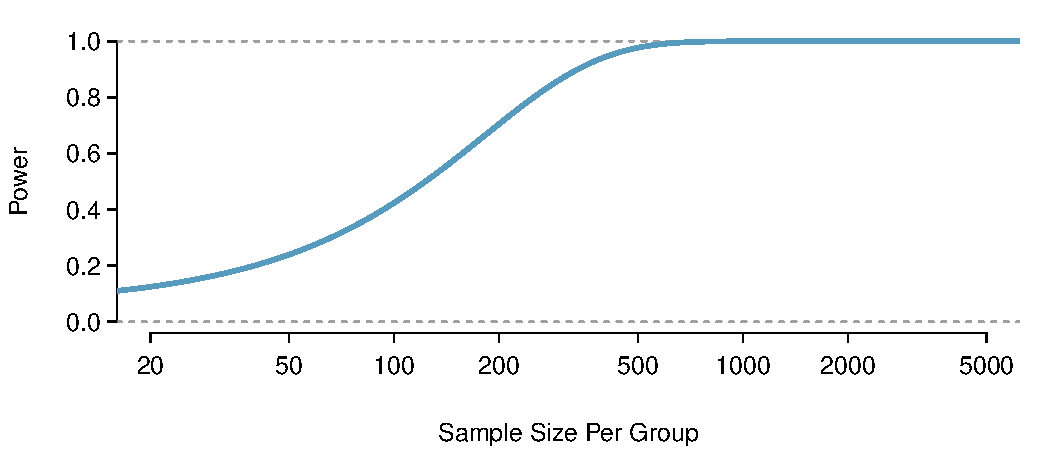
\includegraphics[width=0.80\textwidth]{ch_inference_for_means_oi_biostat/figures/power_curve/power_curve_neg-3}
% \caption{The curve shows the power for different sample sizes in the context of the blood pressure example when the true difference is -3.}
% \label{power_curve_neg-3}
% \end{figure}



% \subsection{Formulas for power and sample size}

% The previous sections have illustrated how power and sample size can be calculated from first principles, using the fundamental ideas behind distributions and testing. In practice, power and sample size calculations are so important that statistical software should be the method of choice; there are many commercially available and public domain programs for performing such calculations. However, hand calculations using formulas can provide quick estimates in the early stages of planning a study.

% Use the following formula to calculate sample size for comparing two means, assuming each group will have $n$ participants:
% \[
% n = \frac{(\sigma_1^2 + \sigma_2^2)( z_{1-\alpha/2} + z_{1-\beta})^2}
% {\Delta^2}.
% \]
% In this formula: 
% \begin{itemize}
% \setlength{\itemsep}{0mm}
	
% 	\item $\mu_1, \mu_2, \sigma_1, \text{ and } \sigma_2$ are the population means and standard deviations of the two groups.
	
% 	\item $\Delta = \mu_1 - \mu_2$ is the minimally important difference that investigators wish to detect.
	
% 	\item The null and alternative hypotheses are $H_0: \Delta = 0$ (i.e., no difference between the means) and $H_A: \Delta \neq 0$, i.e., a two-sided alternative.
	
% 	\item The two-sided significance level is $\alpha$, and $z_{1-\alpha/2}$ is the point on a standard normal distribution with area $1-\alpha/2$ to its left and $\alpha/2$ area to its right.
	
% 	\item $\beta$ is the probability of incorrectly failing to reject $H_0$ for a specified value of $\Delta$; $1- \beta$ is the power.  The value $z_{1-\beta}$ is the point on a standard normal distribution with area $1 - \beta$ to its left.
% \end{itemize}

% %\textD{\newpage}

% For a study with sample size $n$ per group, where $Z$ is a normal random variable with mean 0 and standard deviation 1, power is given by:
% \[
% 	\text{Power } = P\left(  Z <-z_{1 - \alpha/2} + \frac{\Delta}
% 	{\sqrt{\sigma_1^2/n + \sigma_2^2/n}}\right).
% \]

% These formulas could have been used to do the earlier power and sample size calculations for the hypothetical study of blood pressure lowering medication. To calculate the sample size needed for 80\% power in detecting a change of 3 mmHg, $\alpha = 0.05$, $1 - \beta = 0.80$, $\Delta = 3$ mmHg, and $\sigma_1 = \sigma_2 = 12$ mmHg. The formula yields a sample size $n$ per group of 
% \[n = \frac{(12^2 + 12^2)(1.96 + 0.84)^2}{(-3.0)^2} = 250.88, \]
% which can be rounded up to 251.

% The formula for power can be used to verify the sample size of 251:
% \begin{align*}
% 	\text{Power } &= P\left(Z < -1.96 + \frac{3}
% 	{\sqrt{12^2/251 + 12^2/251}}\right) \\
% 	&= P(Z < 1.25) \\
% 	&= 0.85.
% \end{align*}
% The calculated power is slightly larger than 80\% because of the rounding to 251.

% The sample size calculations done before any data are collected are one of the most critical aspects of conducting a study. If an analysis is done incorrectly, it can be redone once the error is discovered. However, if data were collected for a sample size that is either too large or too small, it can be impossible to correct the error, especially in studies with human subjects. As a result, sample size calculations are nearly always done using software. For two-sample $t$-tests, the \textsf{R} function \texttt{power.t.test} is both freely available and easy to use.


%_____________

\section{Notes}
\label{inferenceForNumericalDataNotes}


The material in this chapter is particularly important.  For many applications, $t$-tests and Analysis of Variance (ANOVA), which will study on the next chapter, are an essential part of the core of statistics in medicine and the life sciences.  The comparison of two or more groups is often the primary aim of experiments both in the laboratory and in studies with human subjects. More generally, the approaches to interpreting and drawing conclusions from testing demonstrated in this chapter are used throughout the rest of the text and, indeed, in much of statistics.  

While it is important to master the details of the techniques of testing for differences in two or more groups, it is even more critical to not lose sight of the fundamental principles behind the tests.  A statistically significant difference in group means does not necessarily imply that group membership is the reason for the observed association. A significant association does not necessarily imply causation, even if it is highly significant; confounding variables may be involved. In most cases, causation can only be inferred in controlled experiments when interventions have been assigned randomly. It is also essential to carefully consider the context of a problem. For instance, students often find the distinction between paired and independent group comparisons confusing; understanding the problem context is the only reliable way to choose the correct approach.

It is generally prudent to use the form of the $t$-test that does not assume equal standard deviations, but you have less power.  The formulas are simpler when standard deviations are equal, and software is more widely available for that case.  The differences in sample sizes are usually minor and less important than assumptions about target differences or the values of the standard deviations.  If the standard deviations are expected to be very different, then more specialized software for computing sample size and power should be used. The analysis done after the study has been completed should then use the $t$-test for unequal standard deviations.

Tests for significant differences are sometimes overused in science, with not enough attention paid to estimates and confidence intervals.  Confidence intervals for the difference of two population means show a range of underlying differences in means that are consistent with the data, and often lead to insights not possible from only the test statistic and $p$-value.  Wide confidence intervals may show that a non-significant test is the result of high variability in the test statistic, perhaps caused by a sample size that was too small.  Conversely, a highly significant $p$-value may be the result of such a large sample size that the observed differences are not scientifically meaningful; that may be evident from confidence intervals with very narrow width.

%\textD{\newpage}

Finally, the formula used to approximate degrees of freedom $\nu$ for the independent two-group $t$-test that does not assume equal variance is 
\[\nu = \dfrac{\left[(s_1^2/n_1) + (s_2^2/n_2)\right]^2}{\left[(s_1^2/n_1)^2/(n_1 - 1) + (s_2^2/n_2)^2/(n_2 - 1)\right]}, \]
where $n_1, s_1$ are the sample size and standard deviation for the first sample, and $n_2, s_2$ are the corresponding values for the second sample.
Since $\nu$ is routinely provided in the output from statistical software, there is rarely any need to calculate it by hand.  The approximate formula $\text{df} = \min(n_1 - 1, n_2 - 1)$ always produces a smaller value for degrees of freedom and hence a larger $p$-value.

%The labs for this chapter are structured around particularly important problems in practice: comparing two groups, such as a treatment and control group (Lab 1);  assessing before starting a study whether a sample size is large enough to make it likely that important differences will be detected (Lab 2); comparing more than two groups using analysis of variance (Lab 3); controlling error rates when looking at many comparisons in a dataset (Lab 4); and thinking about hypothesis testing in the larger context of reproducibility (Lab 5). The first four labs provide guidance on how to conduct and interpret specific types of analyses.  Students may find the last lab particularly useful in understanding the distinction between a $p$-value and other probabilities relevant in an inferential setting, such as power.


